\documentclass[tikz]{standalone}
\usepackage{pgfplots}
\usepackage{siunitx}
\usepackage{xcolor}
\pgfplotsset{compat=newest}
\definecolor{light}{HTML}{bdbdbd}
\definecolor{dark}{HTML}{191919}
\begin{document}
\begin{tikzpicture}
	\begin{scope}[scale=0.8]
		\node[scale=0.8, xscale=-1] at (0, 0) {
\includegraphics[width=4cm]{./figures/image-formation/sinogram.png}};
		\draw[-latex] (-2.2, 0) -- ++(4.5, 0) node [right] {\huge \( \theta \)};
		\draw[-latex] (-2, -7) -- ++(0, 14) node [above] {\huge\( r \)};
		\draw (2, 0.2) -- ++(0, -0.4) node [below] {\huge \( \pi \)};
		\node at (-2, 0) [below left] {\huge \( 0 \)};
		\coordinate (20deg low) at (-1.5555556, -6.66);
		\coordinate (130deg high) at (0.8888888, -6.666 + 13.32);
		\draw [red, loosely dashed] (20deg low) -- ++(0, 13.32);
		\draw [red, loosely dashed] (0.8888888, -6.66) -- (130deg high);
	\end{scope}
	\begin{scope}[shift={(7,0)}]
		\begin{scope}[shift={(-70:1cm)}]
			\begin{axis}[
				axis lines=middle, axis line style={-latex},
				anchor={(237,0)}, rotate around={20:(current axis.origin)},
				width=8.18cm, height=3.0cm,
				xlabel={\(r\)}, x label style={rotate=20,below=1mm},
				ylabel={\(\tilde{F}(r, \SI{20}{\degree})\)}, y label style={rotate=20,above=0mm},
				enlarge x limits=0.05,
				enlarge y limits=0.2,
				xtick=\empty,
				ytick=\empty,
			]
			\addplot[color=black,smooth] table[col sep=comma, header=false, x index=0, y index=1] {./figures/image-formation/radon_filtered.csv};
			\end{axis}
		\end{scope}
		\draw[gray, dashed] (-2.35, -0.45) -- ++(-70:4.7cm);
		\draw[gray, dashed] (2.35, -0.57) -- ++(-70:3cm);
		\node at (0, 0) {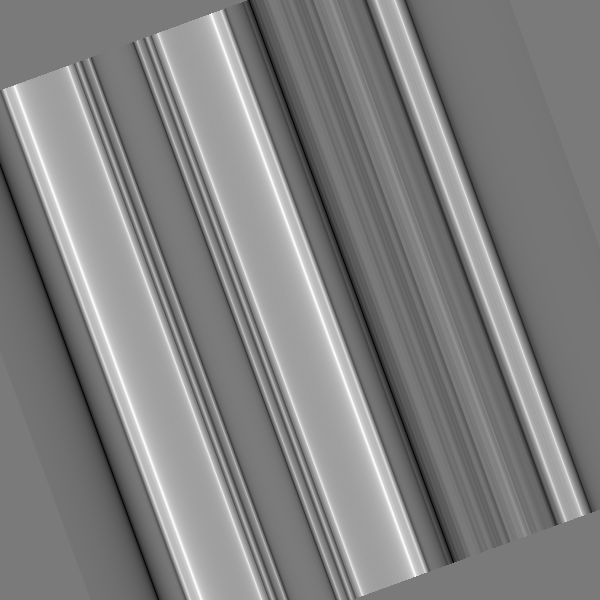
\includegraphics[trim=0cm 6cm 0cm 6cm, clip, width=6cm]{./figures/image-formation/fbp20.png}};
		\draw[-latex] (0, 0) -- ++(4, 0) node [right] {\( x_1 \)};
		\draw[-latex] (0, 0) -- ++(0, 2) node [above] {\( x_2 \)};
		\draw[red] (2.21, -0.72) circle (0.3);
	\end{scope}

	\begin{scope}[shift={(16,0)}]
		\begin{scope}[shift={(40:-7cm)}]
			\begin{axis}[
				axis lines=middle, axis line style={-latex},
				anchor={(185,0)}, rotate around={-50:(current axis.origin)},
				width=8.15cm, height=3cm,
				xlabel={\(r\)}, x label style={rotate=-40,below=1mm},
				ylabel={\(\tilde{F}(r, \SI{130}{\degree})\)}, y label style={rotate=-50,above=0mm},
				enlarge x limits=0.05,
				xtick=\empty,
				ytick=\empty,
			]
			\addplot[color=black,smooth] table[col sep=comma, header=false, x index=0, y index=2] {./figures/image-formation/radon_filtered.csv};
			\end{axis}
		\end{scope}
		\draw[gray, dashed] (-2.35, 0.45) -- ++(40:5.9cm);
		\draw[gray, dashed] (2.35, -0.85) -- ++(40:4cm);
		\node at (0, 0) {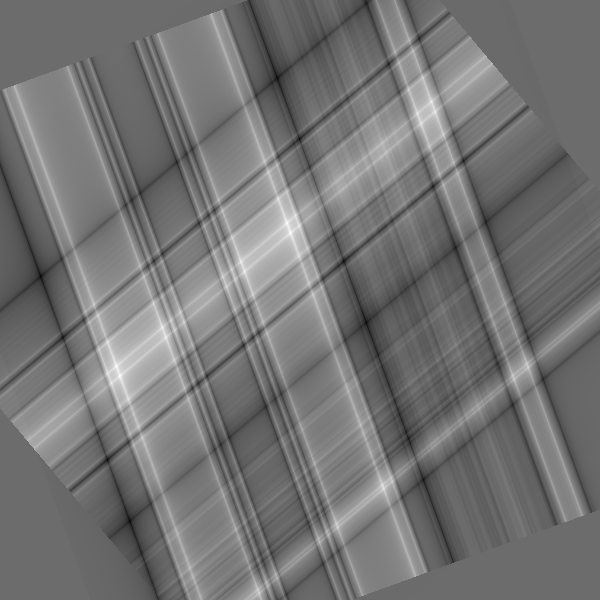
\includegraphics[trim=0cm 6cm 0cm 6cm, clip, width=6cm]{./figures/image-formation/fbp130.png}};
		\draw[-latex] (0, 0) -- ++(4, 0) node [right] {\( x_1 \)};
		\draw[-latex] (0, 0) -- ++(0, 2) node [above] {\( x_2 \)};
		\draw[red] (2.21, -0.72) circle (0.3);
	\end{scope}
	\begin{scope}[shift={(25,0)}]
		\node at (0, 0) {
\includegraphics[trim=0cm 6cm 0cm 6cm, clip, width=6cm]{./figures/image-formation/fbpfull.png}};
		\draw[red] (2.21, -0.72) circle (0.3);
		\draw[-latex] (0, 0) -- ++(4, 0) node [right] {\( x_1 \)};
		\draw[-latex] (0, 0) -- ++(0, 2) node [above] {\( x_2 \)};
	\end{scope}
	\node (f11) at (8, 6) {\( \mathcal{F}_1^{-1} \big\{|\rho| \mathcal{F}_1 \{\cdot\}\big\} \)};
\node (f12) at (3, -7) {\( \mathcal{F}_1^{-1}\big\{ |\rho| \mathcal{F}_1 \{\cdot\}\big\}\)};
	\draw [-latex] (20deg low) to[out=-60, in=180] (f12) to[out=6, in=-110] ++(5, 3);
	\draw [-latex] (130deg high) to[out=60, in=180] (f11) to[out=-10, in=180] ++(9, -1.7);
\end{tikzpicture}
\end{document}
